\newpage
\section{Computer Simulations}

The theory of classical mechanics is often regarded as the first major breakthrough in
the field of physics. For every aspiring physicist this is still the starting point of
their studies. Unfortunately, getting to know these relatively simple laws of nature,
leads to the inescapable realisation that these theories are expressed in mathematical
formalisms that are only analytically solvable in few idealised scenarios. Applying these
formulas to a problem consisting of just more then two particles already leads to
practically unsolvable equations.\\

Although it is often times not possible to find an exact solution to equations
related to complex physical systems, finding reasonable approximations to their solution
is achievable. One popular method to analyse the dynamics of complex systems is the use
of simulations.\\

\begin{wrapfigure}{r}{0.5\textwidth}
  \begin{center}
    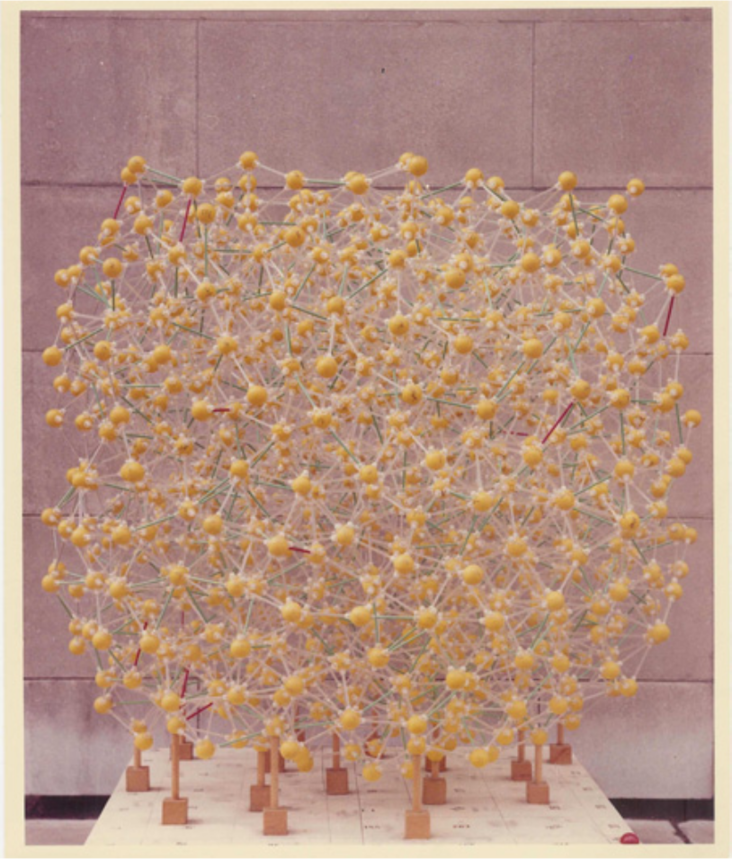
\includegraphics[width=0.38\textwidth]{Figures/WaterModel.png}
  \end{center}
  \caption{Example of an expanded model of a simple liquid (J L Finney, Ph.D thesis)}
\end{wrapfigure}

Simulations have a rich history within physics and engineering, starting even before the
invention of the computer.

An example of one of these mechanical simulations is the Waterloopkundig Laboratorium
or
currently the waterloopbos, a scale model of important
Dutch waterways, where the influence of waves on harbours and docks was studied. This
simulation provided revolutionary insights into the behaviour of water and played an
important part in the design of the famous Delta Works.\\

Another more relevant example is the use of mechanical simulations to study the
structure of water.  In the early 20th century physicist J.D. Bernal and his fellow
researchers build various ball and stick models of water to analyse the possible 3D
configurations of water molecules in a liquid. Their research eventually explained the
peculiar physical properties of water from a atomistic perspective. However useful these
mechanical simulations turned out to be, the biggest drawback of the method was the
extreme cost of labour involved with their construct. As Bernal alluded to in his
famous 1962 lecture,

\begin{quote}
\dots I took a number of rubber balls and stuck them together with rods of a
selection of different lengths ranging from 2.75 to 4 inch. I tried to do this in the
first place as casually as possible, working in my own office being interrupted every
five minutes or so and not remembering what I had done before the interruption.\dots
\end{quote}

After the first computer simulations where performed in the Los Alamos labs, the
popularity of simulations rapidly increased. The remarkable explanatory power of
simulations, combined with the relative easy construction of computer models, lead to a
fast adoption of computer simulations in the scientific community. Within the context of
this thesis, computer simulations are used to study the mechanics of
the DNA polymer. Due to the high number of atoms in a typical system, it is generally
not possible to find an analytical solution to their equations of motion. In this
context, simulations are often used to gain an insight into the complex dynamics of the
system and guide the developments of more simple approximate theories. The simulations
act as a bridge between the microscopic constituents of the systems and the macroscopic
properties we want to understand.


\subsection{Molecular Dynamics Simulations}
Molecular Dynamics (MD) is a computer simulation technique, used to analyse
the dynamics of a classical many-body system. The central idea of this method is to
generate all the trajectories in a system of $N$ particles by numerically
integrating the classical equations of motion,
\[
m_i \frac{d^2 \boldsymbol{r_i}}{dt^2} = \boldsymbol{f_i}, \quad \boldsymbol{f_i} = -
    \frac{\partial}{\partial \boldsymbol{r_i}} \mathcal{U}_i, \quad for\ i \in N.
\]
The motion of the particles are governed by the forces $f_i$ acting upon them, which are
usually derived from the interaction potentials $U_i$.
Solving these differential equations is achieved by employing a discretized time
integration scheme.  Algorithm 1 shows the typical structure of a molecular dynamics
simulation. The discretization resolution is conventionally called the time step of the
simulations denoted by $\Delta t$.\\

\noindent There are a large number of different integrations schemes that one can choose
from, where the choice depends entirely on the system at hand.
When working with an isolated system -- i.e. microcanonical ensemble --, logically an
energy conserving integrator is needed. The canonical
choice for this type of integration scheme is the Velocity-Verlet algorithm. This
algorithm is an example of leapfrog integration, where the updating of the positions
and velocities are interleaved at different points in time. The major strength of this
type of algorithm is that it turns out to be a symplectic integrator, which means the
errors on the conserved energy are bounded.

On the other hand, when a system is in contact with a thermal reservoir --i.e. canonical
ensemble-- not the total energy is conserved, but rather the temperature of the
simulation is fixed. To achieve this, a thermostat is implemented in the MD
simulation. A typical thermostat attempts to negate any drift in temperature by
appropriately importing or exporting energy to the system after each timestep.
Poplular examples of thermostats are the Nos\'e-Hoover thermostat or the Langevin
thermostat.  The latter regulates the temperature by introducing an implicit solvent to
the simulation that gives rise to random thermal kicks. The resulting equations of motion
are the Langevin equations given by,

\begin{equation}
    m_i \frac{d^2 \boldsymbol{r}_i}{dt^2} = - \nabla \mathcal{U}_i - \gamma_i \frac{d
    \boldsymbol{r}_i}{d t} +
    \xi_i(t),
\end{equation}
where $\gamma_i$ is known  as the friction coefficient and $\xi_i(t)$ a random force
acting upon the particles. The combination of the last two terms fully capture the
statistical consequences of the solvent interacting with the system.


\begin{algorithm}
    \SetKwFunction{isOddNumber}{isOddNumber}
    \SetKwInOut{KwIn}{Input}

    \KwIn{Configuration of the system at $t=0$}

    $newList = [\ ]$

    \tcc{For odd elements in the list, we add 1, and for even elements, we add 2.}

    \For{$i \leftarrow 0$ \KwTo $n-1$}{
        \eIf{$\isOddNumber(a_i)$}{

            $newList.append(a_i + 1)$ \tcp*[f]{Some thought-provoking comment.}
         }{
            \tcp{Another comment}
            $newList.append(a_i + 2)$
         }
    }

    \KwRet{$newList$}
    \caption{The Velocity Verlet algorithm}
\end{algorithm}

% \begin{center}
% 	\begin{tikzpicture}[
% 	squarednode/.style={rectangle, draw=blue!60, fill=blue!5, very thick, minimum width=50mm,
% 	minimum height=5mm},]
% 	%Nodes
% 	\node[squarednode]      (step1)                        {1};
% 	\node[squarednode]      (step2)       [below= 3mm of step1] {2};
% 	\node[squarednode]      (step3)       [below= 3mm of step2] {3};
% 	\node[squarednode]      (step4)       [below= 3mm of step3] {4};
% 	\node[squarednode]      (step5)       [below= 3mm of step4] {5};
% 	\node[squarednode]      (step6)       [below= 3mm of step5] {6};
% 	\node[squarednode]      (step7)       [below= 3mm of step6] {7};
% 	\node[squarednode]      (step8)       [below= 3mm of step7] {8};
%
% 	%Lines
%     \draw[very thick, ->] (step1.south) -- (step2.north);
% 	\draw[very thick, ->] (step2.south) -- (step3.north);
% 	\draw[very thick, ->] (step3.south) -- (step4.north);
% 	\draw[very thick, ->] (step4.south) -- (step5.north);
%     \draw[very thick, ->] (step5.south) -- (step6.north);
% 	\draw[very thick, ->] (step6.south) -- (step7.north);
% 	\draw[very thick, ->] (step7.south) -- (step8.north);
% 	\draw[very thick, ->] (step8.west)  -- +(-0.4,0) |-(step2.west);
% 	\end{tikzpicture}
% \end{center}

\subsection{Coarse Grained modelling}
As most thing do, molecular dynamics simulations have their pitfalls. A commonly
encountered problem is the rapidly increasing computational cost, when the number of
particles in the system increase. If not addressed, this would limit the scope of MD
simulations to systems of a few particles over short time-scales.\\

During these simulations the most costly calculations involve the non-bonded
interactions in the system. These interatomic interactions make the computational
complexity for rudimentary MD simulations scale as $O(N^2t)$, where $N$ is the number of
particles in the system and $t$ the simulation time. This bad scaling behaviour comes
from the fact, that for each individual particle all the other particles are contributing
to its interaction potential. To improve this scaling behaviour, the non-bonded
interactions in a MD simulation are almost always truncated. This localization of the
interatomic interactions has the nice effect that not all atoms are involved in every
calculation. Efficient algorithms, like the multigrid method, have been derived to
improve the scaling complexity of MD simulations up to $O(Nt)$.\\

Coarse graining is a method to further optimize molecular dynamics simulations.
In contrary to all atom simulations, where each atom is explicitly represented in the
simulation, in coarse grained simulations multiple atoms are grouped together to form
generalised pseudo-atoms with their respective pseudo-interaction.

There are two distinctly different ways to construct a coarse grained model. The first
method starts from the all atom model of the system and generalises nearby atoms into
larger pseudo-atoms, this is called the bottom up approach. The second method focuses
more on the precise reproduction of a system's thermodynamical properties, rather than
the precise small scale dynamics. Here larger pseudo-atoms are designed, based upon
repeating structures in the system, after which the pseudo-interactions are tweaked to
accurately reproduce the system's dynamics.

In the case of DNA simulations, coarse graining turned out to be a very important method.
Previous all atom simulations of DNA polymers were restricted to simulations of less then
hundred baisepairs over only a few microseconds. Studying large scale systems, often
encountered in DNA technology, was only possible after the development of coarse grained
models. A few examples of commonly used coarse grained models of DNA are Martini, 3SPN
and oxDNA.

\begin{figure}[htpb]
    \centering
    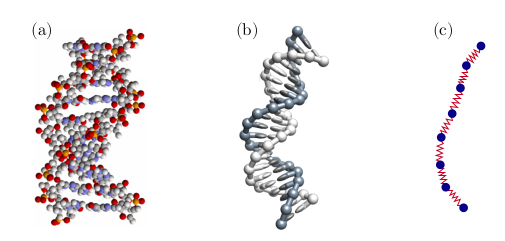
\includegraphics[width=0.6\linewidth]{Figures/CoarseGrained.png}
    \caption{zelf nog maken}%
    \label{fig:Figures/CoarseGrained}
\end{figure}
